\subsection{Why seiyuu?}
\begin{frame}{Why seiyuu?}
\begin{itemize}
\item Because I \textbf{really} like anime and manga.

\item There are many researches whose focus is actor's social network but usually is hollywood actors and not only voice actors. Seiyuu and anime industry is really unusual and so could present a different structure.

\item There're several database with information about anime and seiyuu but they are either incomplete or don't have a good structure nor format.
\end{itemize}
\end{frame}
%-------------------------------------------------------------------------

\subsection{Wikidata and MyAnimeList}
\begin{frame}{Wikidata and MyAnimeList}
We wanted to use \emph{Wikidata} as our source but it's too incomplete; it doesn't have information about works of seiyuu.
\vspace{15pt}

Instead we used \emph{MyAnimeList} (MAL) through an API called \emph{Jikan}; retrieving data in JSON and then changing its format to RDF.
\vspace{15pt}

We used Wikidata to get the list of seiyuu and MyAnimeList to get list of works for each seiyuu and information about anime.
\end{frame}
%-------------------------------------------------------------------------

\begin{frame}
\begin{center}
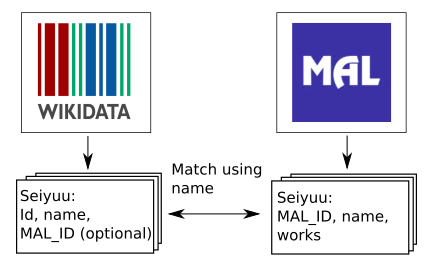
\includegraphics[scale=0.7]{graphics/wikidataMAL.png} 
\end{center}

\begin{itemize}
\item Total of 6472 seiyuu on Wikidata
%There’s actually 7030 seiyuu in wikidata but only 6472 of them have an English label
\item Only 59 had MAL\_IDs
\item 3033 MAL\_IDs retrieved
\item At the end having 3092 seiyuu with MAL\_ID
\item 2956 of which had at least one work

\end{itemize}
\end{frame}
%-------------------------------------------------------------------------

\subsection{Data retrieved}
\begin{frame}{Data retrieved}
All in all we were able to retrieve the following information for \emph{2956 seiyuu and 7614 anime}.

\begin{itemize}
	\item For Seiyuu:
	\begin{itemize}
		\item Name
		\item Debut (this was obtained from oldest work's aired date)
		\item Gender
		\item Popularity (member\_favorites information of MAL)
		\item Works (anime roles with anime information plus wheter is a main role or not)
	\end{itemize}
	\item For Works (Anime):
	\begin{itemize}
		\item Year that began airing
		\item Favorites
		\item Score (from 0 to 10, MAL user based)
		\item Popularity (ranking over all MAL animes)
		\item Members (how many MAL users have it on their list)
		\item Genres
	\end{itemize}
\end{itemize}
\end{frame}